\chapter{Convolutional Neural Networks}
Convolutional Neural Network is a class of deep, feed-forward neural network, that can be successfully applied to systems with high dimensional input such as images.

It is a pattern recognition mechanisms that is inspired by the way in which mammals visually perceive the world around them using a layered architecture of neurons in the brain. 

Convolutional Neural Networks leverage three ideas:
\begin{enumerate}
\itemsep0em 
\item local connectivity
\item parameter sharing
\item pooling hidden units
\end{enumerate}

CNNs exploit spatially-local correlation by enforcing a local connectivity pattern between neurons of adjacent layers. In other words, each unit in the convolutional hidden layer is not connected with all units in a previous layer, instead it is connected to a subset of units from a previous layer. This approach helps to solve the problem of unmanageable number of parameters. 


The primary purpose of convolution in case of a CNNs is to extract features from the input image. In convolutional layer, the set of filters (typically square matrices with random values) is generated. 

Each filter $h_{i}$ is replicated across the entire visual field. These replicated units share the same parameterization (weight vector and bias) and form a feature (activation) map. Activation maps indicate ‘activated’ regions, i.e. regions where features specific to the filter have been detected in the input. 

Computation of those feature maps corresponds to computation of discrete convolution of a $i_{th}$ channel of input and filter matrix $W_{ij}$. The activation function is applied to the convolution result.

That is how the next hidden layer is computed using ReLU as an activation function:

\begin{equation}
y_{i} = ReLU(\sum_{i} k_{ij} \cdot x_{i})
\end{equation}

The values of the filter matrix change with each learning iteration over the training set, indicating that the network is learning to identify which regions are of significance for extracting features from the data. The training process is called backpropagation and is described in chapter (TODO ???).

Another important concept of CNNs is max-pooling, which is a form of non-linear down-sampling. Max-pooling partitions the input image into a set of non- overlapping rectangles and, for each such subregion, outputs the maximum value.
Max-pooling is useful in vision for two reasons: 

\begin{itemize}
\itemsep0em 
\item By eliminating non-maximal values, it reduces computation for upper layers.
\item It provides a form of translation invariance.
\end{itemize}

Since it provides additional robustness to position, max-pooling is a “smart” way of reducing the dimensionality.
\\\\\\\\
After a sequence of those operation the output is flattened and applied to the fully connected layer.
At the very end of the network the output is squashed with the softmax layer, so that each element in the output vector corresponds to the probability value for each class.

\begin{equation}
\sigma(o_{j}) = \frac{e^{o_{j}}}{\sum_{k=1}^{K} e^{o_{k}}}
\end{equation}

where $K$ is the number of classes and $o_{j}$ is the $j_{th}$ value of the output vector.

The whole process is presented in the figure (??) 

\begin{figure}[H]
\centering
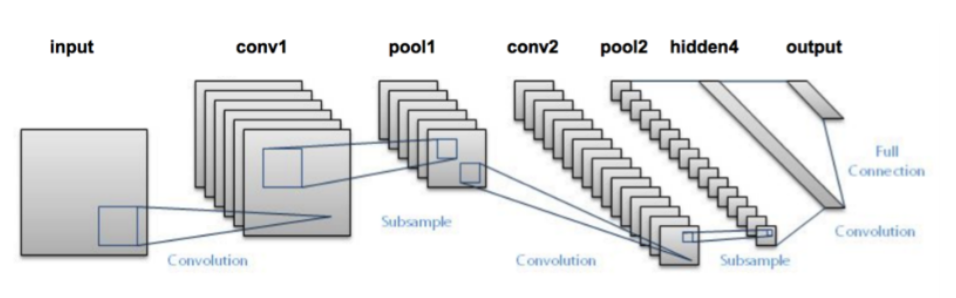
\includegraphics[scale=0.7]{img/proces.png}
\caption{A typical convolutional neural network for face recognition}
\end{figure}

DeepFace [Taigman et al., 2014] and FaceNet [Schroff, Kalenichenko, and Philbin, 2015] are two of the most successful applications of CNNs in the Face Recognition  problem. These two have provided state-of-art results in recent years, with the best results being obtained by the second one.

\section{Implementation and test results}

The Convolutional Neural Network may differ in number of layers and their connections. The one that was implemented has the following architecture:

\begin{python}
    def forward_pass(self, X):
        h = self.relu(self.cnn_layer(X, layer_i=0, border_mode="full"))
        h = self.relu(self.cnn_layer(h, layer_i=1, border_mode="valid"))
        h = self.maxpooling_layer(h)
        h = self.relu(self.cnn_layer(h, layer_i=3, border_mode="valid"))
        h = self.maxpooling_layer(h)
        h = self.flatten_layer(h)
        h = self.relu(self.dense_layer(h, layer_i=6))
        h = self.dense_layer(h, layer_i=7)
        h = self.softmax_layer2D(h)
        max_i = self.classify(h)
      	return max_i[0]
\end{python}


\subsection{Convolutional layers}

The first two and the 4th layer in the network performs the convolutional operation followed by activation function RELU.

The input to the network is an image, that can be treated as matrix with three dimensions, each corresponding to every color channel (RGB). In this case every image has the same width and height $k$ equal to 76 pixels. 

\begin{equation}
R =
\left[
\begin{matrix}
r_{11} & r_{21} & \cdots & \cdots & r_{k1}\\
r_{12} & r_{22} & \cdots & \cdots & r_{k2}\\
r_{13} & r_{23} & \cdots & \cdots & r_{k3}\\
r_{14} & r_{24} & \cdots & \cdots & r_{k4}\\
\cdots & \cdots & \cdots & \cdots & \cdots\\
\cdots & \cdots & \cdots & \cdots & \cdots\\
r_{1k} & r_{2k} & \cdots & \cdots & r_{kk}
\end{matrix}
\right]
G =
\left[
\begin{matrix}
g_{11} & g_{21} & \cdots & \cdots & g_{k1}\\
g_{12} & g_{22} & \cdots & \cdots & g_{k2}\\
g_{13} & g_{23} & \cdots & \cdots & g_{k3}\\
g_{14} & g_{24} & \cdots & \cdots & g_{k4}\\
\cdots & \cdots & \cdots & \cdots & \cdots\\
\cdots & \cdots & \cdots & \cdots & \cdots\\
g_{1k} & g_{2k} & \cdots & \cdots & g_{kk}
\end{matrix}
\right]
B =
\left[
\begin{matrix}
b_{11} & b_{21} & \cdots & \cdots & b_{k1}\\
b_{12} & b_{22} & \cdots & \cdots & b_{k2}\\
b_{13} & b_{23} & \cdots & \cdots & b_{k3}\\
b_{14} & b_{24} & \cdots & \cdots & b_{k4}\\
\cdots & \cdots & \cdots & \cdots & \cdots\\
\cdots & \cdots & \cdots & \cdots & \cdots\\
b_{1k} & b_{2k} & \cdots & \cdots & b_{kk}
\end{matrix}
\right]
\end{equation}

In convolutional layer each of those matrices were convolved with each of 32 randomly chosen filters. As result we obtained a matrix with following dimensions: 

\begin{equation}
C ~ (32,32
\end{equation}



 

